\section{Diffusion}
This section discusses the binary limit of the diffusion coefficients in a ternary system. The purpose of the section is to give insight into how the force-flux in a binary system relate to those in a ternary, how to interpret the diffusion coefficients in a ternary system, and raise awareness regarding potential pitfalls when attempting to model a ternary system as a pseudo-binary system.

\subsection{Notation}\label{sec:diffusion_notation}

In the following text, $D_{ii}^{(b)}$ is used to denote the diffusion coefficient of a binary system, where component $i$ is the independent component. $D_{ii}^{(k)}$ denotes the diagonal elements of the Fick diffusion matrix in a ternary system, where component $k$ is the dependent component. $D_{ij}$ denotes the non-diagonal elements of the Fick diffusion matrix in a ternary system, where components $i$ and $j$ are the independent components.

In section \ref{sec:dependent}, $\tilde{D}_{ij}^{(t)}$ and $\tilde{D}_{ij}^{(b)}$ are used to denote the diffusion coefficients corresponding to the linearly dependent formulations of Fick's law.

\subsection{Independent Fluxes}\label{sec:diff_indep}

For a ternary system (1, 2, 3), we can formulate Fick's law for a set of independent fluxes as either

\begin{equation}
    \begin{split}
        \begin{pmatrix}J_1 \\ J_2\end{pmatrix} = \begin{bmatrix}D_{11}^{(3)} & D_{12} \\ D_{21} & D_{22}^{(3)}\end{bmatrix} \begin{pmatrix}\nabla c_1 \\ \nabla c_2\end{pmatrix},
    \end{split}
    \label{eq:tern_dep3}
\end{equation}
\begin{equation}
    \begin{split}
        \begin{pmatrix}J_1 \\ J_3\end{pmatrix} = \begin{bmatrix}D_{11}^{(2)} & D_{13} \\ D_{31} & D_{33}^{(2)}\end{bmatrix} \begin{pmatrix}\nabla c_1 \\ \nabla c_3\end{pmatrix},
    \end{split}
    \label{eq:tern_dep2}
\end{equation}
or
\begin{equation}
    \begin{split}
        \begin{pmatrix}J_2 \\ J_3\end{pmatrix} = \begin{bmatrix}D_{22}^{(1)} & D_{23} \\ D_{32} & D_{33}^{(1)}\end{bmatrix} \begin{pmatrix} \nabla c_2 \\ \nabla c_3\end{pmatrix}.
    \end{split}
    \label{eq:tern_dep1}
\end{equation}
Where the superscript on the diffusion coefficients indicates which component is the dependent component.

For a binary system (1, 2), we can choose between
\begin{equation}
    J_1^{(b)} = D_{11}^{(b)} \nabla c_1
    \label{eq:bin_dep2}
\end{equation}
and
\begin{equation}
    J_2^{(b)} = D_{22}^{(b)} \nabla c_2.
    \label{eq:bin_dep1}
\end{equation}

Now we can examine the question: "When $x_3 \to 0$, and (necessarily) $\nabla c_3 \to 0$ and $J_3 \to 0$, do the ternary coefficients reduce to the corresponding binary coefficients?"

To answer that question, we must be clear about which ternary formulation reduces to which binary formulation.

In the ternary formulation \eqref{eq:tern_dep2}, $J_2$ is the dependent flux, so if $x_3 = \nabla c_3 = 0$ (something we are free to demand, as $\nabla c_1$ and $\nabla c_3$ are independent), $J_1 = D_{11}^{(2)} \nabla c_1$. Thus, we expect that formulation \eqref{eq:tern_dep2} should reduce to formulation \eqref{eq:bin_dep2} when $x_3 = \nabla c_3 = 0$. Therefore, we expect
\begin{equation}
    D_{11}^{(2)}(x_3 = 0) = D_{11}^{(b)}.
\end{equation}

By similar argument, it's formulation \eqref{eq:tern_dep1} that reduces to formulation \eqref{eq:bin_dep1}, so
\begin{equation}
    D_{22}^{(1)}(x_3 = 0) = D_{22}^{(b)}.
\end{equation}

Note that formulation \eqref{eq:tern_dep3} does not immediately reduce to one of the binary formulations when $x_3 \to 0$; this is because in this formulation, we cannot demand $\nabla c_3 = 0$ because component 3 is the dependent component in this formulation. Therefore, the coefficients in formulation \eqref{eq:tern_dep3} cannot be expected to reduce to the binary coefficients when $x_3 \to 0$.

Figure \ref{fig:binary_ternary} shows how the ternary coefficients expected to reduce to the corresponding binary coefficients behave as a function of $x_3$.

\begin{figure}[htb]
    \centering
    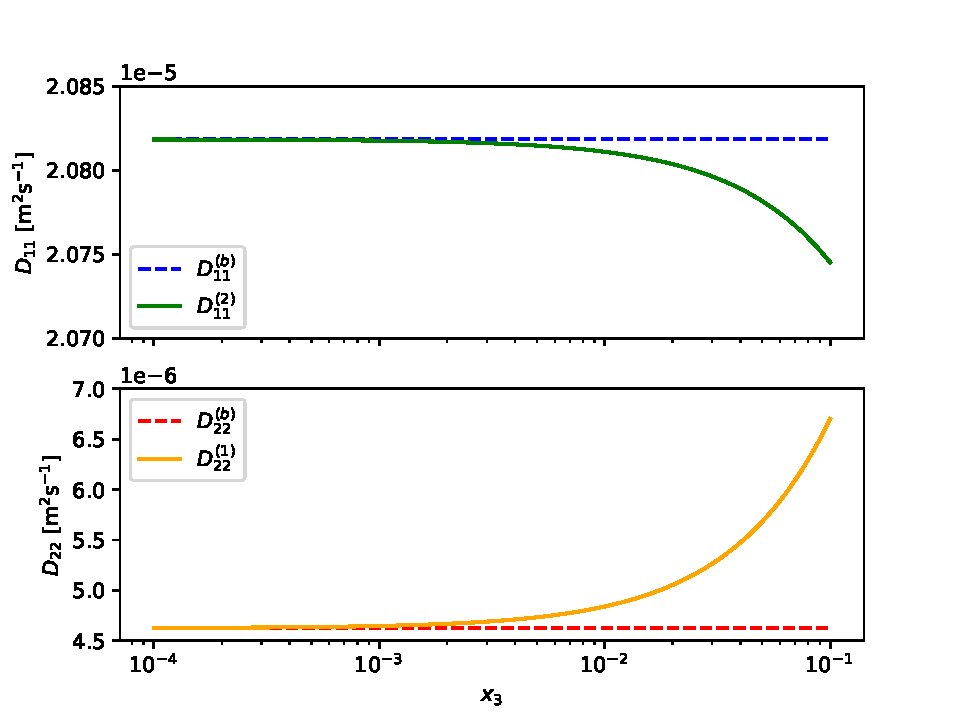
\includegraphics[width=.75\textwidth]{binary_ternary.pdf}
    \caption{The ternary diffusion coefficients reduce to the corresponding binary coefficients when $x_3 \to 0$.}
    \label{fig:binary_ternary}
\end{figure}


\subsection{Dependent Fluxes}\label{sec:dependent}

An alternative flux-force formulation for the ternary system is through a set of \textit{dependent} fluxes and forces; thus, we can formulate Fick's law as

\begin{equation}
    \begin{split}
        \begin{pmatrix}J_1 \\ J_2 \\ J_3 \end{pmatrix} = \begin{bmatrix}\tilde{D}_{11}^{(t)} & \tilde{D}_{12}^{(t)} & \tilde{D}_{13}^{(t)} \\ \tilde{D}_{21}^{(t)} & \tilde{D}_{22}^{(t)} & \tilde{D}_{23}^{(t)} \\ \tilde{D}_{31}^{(t)} & \tilde{D}_{32}^{(t)} & \tilde{D}_{33}^{(t)} \end{bmatrix} \begin{pmatrix}\nabla c_1 \\ \nabla c_2 \\ \nabla c_3\end{pmatrix},
    \end{split}
\end{equation}
and correspondingly for the binary system:
\begin{equation}
    \begin{split}
        \begin{pmatrix}J_1 \\ J_2\end{pmatrix} = \begin{bmatrix}\tilde{D}_{11}^{(b)} & \tilde{D}_{12}^{(b)} \\ \tilde{D}_{21}^{(b)} & \tilde{D}_{22}^{(b)}\end{bmatrix} \begin{pmatrix}\nabla c_1 \\ \nabla c_2\end{pmatrix}.
    \end{split}
\end{equation}

Note that these two matrices are not invertible because they implicitly contain the dependency $J_1 + J_2 + J_3 = 0$. However, this formulation can be useful for consistency checking because when $x_3 \to 0$, Equation \eqref{eq:dep_matr_eqiv} should hold:

\begin{equation}
    \begin{bmatrix}\tilde{D}_{11}^{(t)} & \tilde{D}_{12}^{(t)} \\ \tilde{D}_{21}^{(t)} & \tilde{D}_{22}^{(t)} \end{bmatrix} = \begin{bmatrix}\tilde{D}_{11}^{(b)} & \tilde{D}_{12}^{(b)} \\ \tilde{D}_{21}^{(b)} & \tilde{D}_{22}^{(b)}\end{bmatrix}.
    \label{eq:dep_matr_eqiv}
\end{equation}

This equality should hold precisely because the matrices contain the dependence between the fluxes and forces, and when $x_3 = \nabla c_3 = 0$, $J_1 + J_2 = 0$, and we should obtain the same fluxes as from the binary matrix.

Figure \ref{fig:dependent} demonstrates that Equation \eqref{eq:dep_matr_eqiv} is satisfied when $x_3 \to 0$.

\begin{figure}[bht]
    \centering
    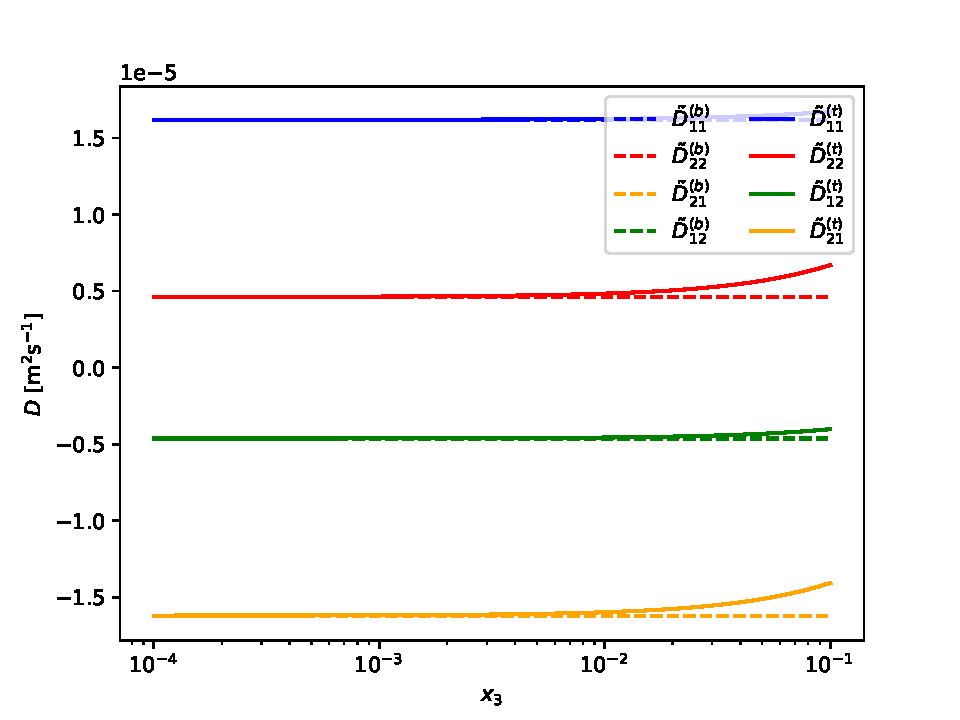
\includegraphics[width=.75\textwidth]{dependent.pdf}
    \caption{The coefficients in the singular, ternary Fick matrix reduce to the corresponding coefficients in the singular, binary Fick matrix when $x_3 \to 0$.}
    \label{fig:dependent}
\end{figure}

Finally, for the ternary matrix, we can observe that
\begin{equation}
    \tilde{D}_{13} - \tilde{D}_{23} = 0
\end{equation}
when $x_3 = 0$ because when $x_3 = \nabla c_3 = 0$, $\nabla c_2 = - \nabla c_1$, and $J_3$ should vanish. Figure \ref{fig:vanish3} demonstrates that this condition is met.

\begin{figure}[bth]
    \centering
    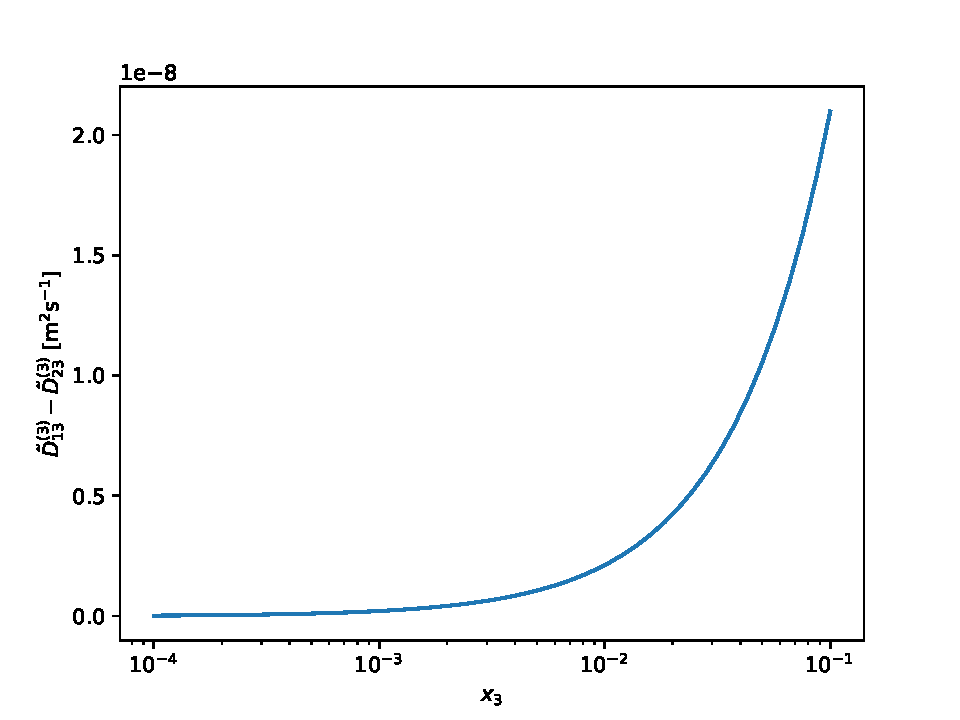
\includegraphics[width=.75\textwidth]{vanish3.pdf}
    \caption{The flux $J_3$ vanishes when $x_3 \to 0$ and $\nabla c_3 = 0$.}
    \label{fig:vanish3}
\end{figure}
